% =====================================================================
%  Slides: ETSI GS QKD 018, SDN orchestration of multi-domain QKD networks
%  ---------------------------------------------------------------------
%  BUILD (plain pdfLaTeX; XeLaTeX/LuaLaTeX also work and use Cambria Math):
%      latexmk -pdf main.tex
%  or by hand:
%      pdflatex main.tex ; biber main ; pdflatex main.tex ; pdflatex main.tex
%  The TikZ figures in figures/ are the paper's (paper/en/figures),
%  without the figure environment, scaled with \slidefig.
% =====================================================================
\documentclass[10pt]{beamer}
% =====================================================================
%  Slide preamble: classic Beamer theme (Warsaw), fonts, listings, TikZ
% =====================================================================

% ---------- Fonts and language ----------
% pdfLaTeX: standard Latin Modern. XeLaTeX/LuaLaTeX: Cambria Math if installed.
\usepackage{iftex}
\ifPDFTeX
  \usepackage[utf8]{inputenc}
  \usepackage[T1]{fontenc}
  \usepackage{lmodern}
  \usepackage{amsmath,amssymb}
\else
  \usefonttheme{professionalfonts}
  \usepackage{fontspec}
  \usepackage{amsmath,amssymb}
  \usepackage{unicode-math}
  \IfFontExistsTF{Cambria Math}
    {\setmathfont{Cambria Math}}
    {\setmathfont{Latin Modern Math}}
\fi
\usepackage[english]{babel}
\usepackage{csquotes}

% ---------- Classic theme ----------
\usetheme{Warsaw}
\setbeamertemplate{navigation symbols}{}
% Split footline as in the theme, with the frame number on the right
\setbeamertemplate{footline}{%
  \leavevmode%
  \hbox{%
  \begin{beamercolorbox}[wd=.5\paperwidth,ht=2.5ex,dp=1.125ex,leftskip=.3cm plus1fill,rightskip=.3cm]{author in head/foot}%
    \usebeamerfont{author in head/foot}\insertshortauthor
  \end{beamercolorbox}%
  \begin{beamercolorbox}[wd=.5\paperwidth,ht=2.5ex,dp=1.125ex,leftskip=.3cm,rightskip=.3cm]{title in head/foot}%
    \usebeamerfont{title in head/foot}\insertshorttitle\hfill\insertframenumber{} / \inserttotalframenumber
  \end{beamercolorbox}}%
  \vskip0pt}

% Outline at the start of each section
\AtBeginSection[]{%
  \begin{frame}<beamer>
    \tableofcontents[currentsection,hideothersubsections]
  \end{frame}}

% ---------- Packages ----------
\usepackage{booktabs,tabularx,array}
\usepackage{listings}
\usepackage{adjustbox}
\usepackage{tikz}
\usetikzlibrary{arrows.meta,positioning,fit,calc,shapes.geometric,backgrounds}
\usepackage[backend=biber,style=numeric-comp,sorting=none,maxbibnames=3,
            url=false,doi=false,eprint=false,isbn=false]{biblatex}
\addbibresource{bibliography/references.bib}
\renewcommand*{\bibfont}{\scriptsize}
\setbeamertemplate{bibliography item}{\insertbiblabel}
\newcolumntype{L}{>{\raggedright\arraybackslash}X}

% ---------- Listings (YANG, pyang trees, HTTP) ----------
\lstdefinelanguage{yang}{
  morekeywords={module,namespace,prefix,import,organization,contact,
    description,revision,reference,yang-version,identity,base,typedef,type,
    identityref,grouping,uses,container,list,key,leaf,leaf-list,config,
    augment,rpc,input,output,notification,leafref,path,default,units,
    must,when,enum,enumeration,mandatory},
  sensitive=true,
  morecomment=[l]{//},
  morecomment=[s]{/*}{*/},
  morestring=[b]"
}
\lstset{
  basicstyle=\ttfamily\scriptsize,
  keywordstyle=\bfseries,
  frame=single,
  columns=fullflexible, keepspaces=true,
  breaklines=true, upquote=true,
  aboveskip=4pt, belowskip=4pt
}

% ---------- Common TikZ styles (as in the paper) ----------
\tikzset{
  >=Stealth,
  box/.style={draw,rounded corners,minimum height=8mm,align=center,
              font=\small},
  lbl/.style={font=\scriptsize,midway,fill=white,inner sep=1pt},
  actor/.style={draw,rounded corners,fill=gray!8,minimum width=2.4cm,
                minimum height=7mm,align=center,font=\small},
  msg/.style={->,thick},
  ret/.style={->,dashed}
}

% Paper TikZ figure scaled to the slide: \slidefig[max height]{file}
\newcommand{\slidefig}[2][0.75\textheight]{%
  \begin{center}
    \begin{adjustbox}{max width=\textwidth,max totalheight=#1}
      \input{figures/#2}
    \end{adjustbox}
  \end{center}}

% Source note, bottom right
\newcommand{\source}[1]{\vfill\hfill{\tiny #1}}


\title[ETSI GS QKD 018]{SDN Orchestration of Multi-Domain QKD Networks}
\subtitle{The ETSI GS QKD 018 Interface}
\author[D.~Carro, F.~E.~Bucci]{Diego Carro \and Bucci Felice Elia}
\institute[PoliTo]{Cybersecurity course, Politecnico di Torino\\Quantum Engineering}
\date{November 2026}

\begin{document}

% ---------------------------------------------------------------------
\begin{frame}
  \titlepage
\end{frame}

\begin{frame}{Outline}
  \tableofcontents[hideallsubsections]
\end{frame}

% =====================================================================
\section[Introduction]{Introduction: from QKD to the network}
% =====================================================================

\subsection{Motivation}

\begin{frame}{The problem}
  \begin{itemize}
    \item QKD lets two parties agree on a secret key whose security rests
          on \alert{physics}, not on computational hardness.
    \item Bringing it into an operator network means managing it like any
          other \alert{network resource}:
          \begin{itemize}
            \item discover its topology and monitor its state;
            \item allocate its capacity to services;
            \item coordinate it with the classical optical network.
          \end{itemize}
    \item The ETSI ISG QKD tackled the problem step by step:
  \end{itemize}
  \vspace{1ex}
  \begin{center}
  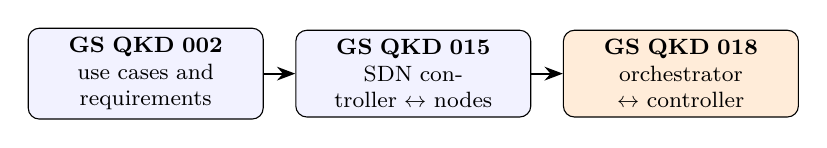
\begin{tikzpicture}[node distance=4mm,
      st/.style={draw,rounded corners,fill=blue!5,align=center,
                 font=\footnotesize,minimum height=11mm,text width=2.75cm}]
    \node[st] (a) {\textbf{GS QKD 002}\\use cases and requirements};
    \node[st,right=of a] (b) {\textbf{GS QKD 015}\\SDN controller $\leftrightarrow$ nodes};
    \node[st,right=of b,fill=orange!15] (c) {\textbf{GS QKD 018}\\orchestrator $\leftrightarrow$ controller};
    \draw[->,thick] (a) -- (b);
    \draw[->,thick] (b) -- (c);
  \end{tikzpicture}
  \end{center}
\end{frame}

\begin{frame}{State of the art in brief}
  \small
  \begin{columns}[T]
    \begin{column}{0.5\textwidth}
      \begin{block}{Foundations and networks}
        \begin{itemize}
          \item Review of protocols and security proofs~\cite{pirandola2020}
          \item From link to network: layers, trusted relay,
                routing~\cite{mehic2020,cao2022,routing2024}
        \end{itemize}
      \end{block}
      \begin{block}{Standards}
        \begin{itemize}
          \item ETSI: use cases~\cite{qkd002}, APIs~\cite{qkd004,qkd014},
                SDN~\cite{qkd015}, orchestration~\cite{qkd018}, KMS~\cite{qkd020}
          \item ITU-T Y.3800: architecture, control, SDN~\cite{ituy3800,ituy3804,ituy3805}
        \end{itemize}
      \end{block}
    \end{column}
    \begin{column}{0.5\textwidth}
      \begin{block}{SDN and orchestration}
        \begin{itemize}
          \item First SDN + QKD experiments (UPM/Telefónica)~\cite{aguado2016,aguado2020}
          \item KOREN multi-vendor (SK Telecom)~\cite{sim2023}
          \item Hierarchical ONOS prototype (PoliMi)~\cite{vicario2025}
          \item MadQCI, Madrid~\cite{madqci2024}
        \end{itemize}
      \end{block}
      \begin{exampleblock}{Contribution}
        A unified reading of the 002 $\to$ 015 $\to$ 018 chain: from
        requirements to YANG models to multi-domain orchestration.
      \end{exampleblock}
    \end{column}
  \end{columns}
\end{frame}

\subsection{QKD and trusted nodes}

\begin{frame}{Quantum key distribution}
  \begin{columns}[T]
    \begin{column}{0.56\textwidth}
      \textbf{BB84 in four steps}
      \begin{enumerate}
        \item Alice encodes random bits on single photons, in one of two
              randomly chosen bases.
        \item Bob measures in a random basis.
        \item Over an \alert{authenticated} classical channel they compare
              bases (\emph{sifting}).
        \item Error correction and \emph{privacy amplification} distil the
              key.
      \end{enumerate}
      \vspace{1ex}
      An eavesdropper introduces measurable errors:
      \[
        \mathrm{QBER} = \frac{N_{\text{errors}}}{N_{\text{sifted}}}
        \lesssim 11\% \ \text{(BB84)}
      \]
    \end{column}
    \begin{column}{0.42\textwidth}
      \begin{block}{What the network cares about}
        The \emph{secret key rate} (SKR), in bit/s, drops with distance:
        \[
          \eta = 10^{-\alpha L/10}
        \]
        with \(\alpha \approx 0.2\)~dB/km.
      \end{block}
      \begin{alertblock}{Two remarks}
        \begin{itemize}
          \item QKD \emph{distributes} keys; it neither encrypts nor
                authenticates.
          \item It needs an initial secret: it is \emph{key growing}.
        \end{itemize}
      \end{alertblock}
    \end{column}
  \end{columns}
\end{frame}

\begin{frame}{From link to network: the trusted node}
  \begin{columns}[c]
    \begin{column}{0.52\textwidth}
      \begin{itemize}
        \item A link spans at most a few hundred km; practical quantum
              repeaters do not exist yet.
        \item Real networks chain links through \alert{trusted nodes}.
        \item Each hop is a one-time pad, but $K$ is in the clear inside
              every intermediate node.
        \item Relaying \alert{consumes key}: each link $\ell\in p$ spends
              $|K|$ bits. Key becomes a resource to be planned.
      \end{itemize}
    \end{column}
    \begin{column}{0.46\textwidth}
      \begin{center}\begin{adjustbox}{max width=\linewidth}
      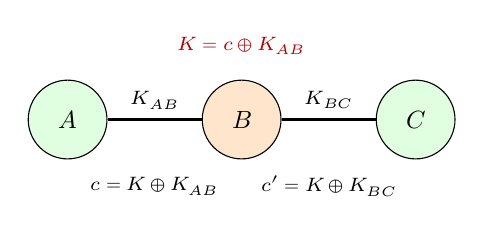
\begin{tikzpicture}[scale=0.85,
          nd/.style={draw,circle,fill=green!12,minimum size=10mm,font=\small}]
        \node[nd] (A) at (0,0) {$A$};
        \node[nd,fill=orange!20] (B) at (2.6,0) {$B$};
        \node[nd] (C) at (5.2,0) {$C$};
        \draw[thick] (A) -- node[above,font=\scriptsize]{$K_{AB}$} (B);
        \draw[thick] (B) -- node[above,font=\scriptsize]{$K_{BC}$} (C);
        \node[font=\scriptsize,align=center] at (1.3,-1.0) {$c = K\oplus K_{AB}$};
        \node[font=\scriptsize,align=center] at (3.9,-1.0) {$c' = K\oplus K_{BC}$};
        \node[font=\scriptsize,align=center,red!70!black] at (2.6,1.1)
             {$K = c\oplus K_{AB}$};
      \end{tikzpicture}
      \end{adjustbox}\end{center}
    \end{column}
  \end{columns}
\end{frame}

\subsection{Architecture and SDN}

\begin{frame}{The ITU-T Y.3800 layered architecture}
  \slidefig[0.55\textheight]{itu_layers}
  \small
  \begin{columns}[T]
    \begin{column}{0.5\textwidth}
      \textbf{QKD link}: two QKD modules, where key is \emph{generated}.\\
      \textbf{KM link}: two key managers, where key is \emph{relayed}.
    \end{column}
    \begin{column}{0.5\textwidth}
      \textbf{QKDN controller}: acts in real time (paths, links).\\
      \textbf{QKDN manager}: supervises (FCAPS, policies).
    \end{column}
  \end{columns}
  \source{Adapted from ITU-T Y.3800~\cite{ituy3800}}
\end{frame}

\begin{frame}{Software-Defined Networking}
  \begin{columns}[c]
    \begin{column}{0.5\textwidth}
      \begin{itemize}
        \item SDN separates the \emph{data plane}, the \emph{control
              plane} (a controller with a global view) and the
              \emph{application plane}~\cite{kreutz2015}.
        \item The controller talks to devices through the \alert{SBI} and
              offers services upwards through the \alert{NBI}.
        \item With several domains, an \alert{orchestrator} sits on top.
      \end{itemize}
      \vspace{1ex}
      \small A QKD network has everything that makes SDN useful: scarce and
      variable resources, physical constraints, multi-vendor equipment,
      changing demand.
    \end{column}
    \begin{column}{0.46\textwidth}
      \begin{center}
      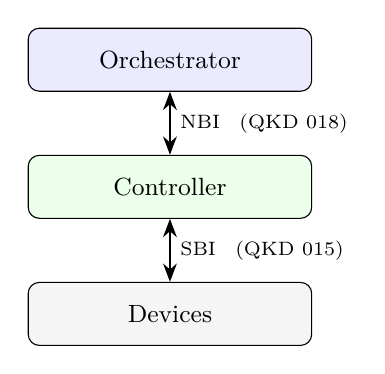
\begin{tikzpicture}[node distance=8mm]
        \node[box,fill=blue!8,minimum width=3.6cm] (o) {Orchestrator};
        \node[box,fill=green!8,minimum width=3.6cm,below=of o] (c) {Controller};
        \node[box,fill=gray!8,minimum width=3.6cm,below=of c] (d) {Devices};
        \draw[<->,thick] (o) -- node[right,font=\scriptsize]{NBI\quad(QKD 018)} (c);
        \draw[<->,thick] (c) -- node[right,font=\scriptsize]{SBI\quad(QKD 015)} (d);
      \end{tikzpicture}
      \end{center}
    \end{column}
  \end{columns}
\end{frame}

% =====================================================================
\subsection{GS QKD 002}
% =====================================================================

\begin{frame}{GS QKD 002 (2010): where QKD is needed}
  \begin{columns}[T]
    \begin{column}{0.48\textwidth}
      \begin{block}{One primitive out of three}
        A secure system needs \emph{encryption}, \emph{key distribution}
        and \emph{authentication}. QKD covers \alert{only the second}: it
        complements classical cryptography (OTP/AES, Wegman–Carter MACs)
        rather than replacing it.
      \end{block}
    \end{column}
    \begin{column}{0.5\textwidth}
      \textbf{Where the key is consumed}
      \begin{description}\small
        \item[L2] PPP, MACsec, QKD link encryptor
        \item[L3] modified IKE for IPsec
        \item[L4] TLS session keys, HMAC
        \item[L7] application-level authentication and encryption
      \end{description}
      \small In every case there is a key \emph{consumer} and a key
      \emph{provider}: the future \alert{SAE / KME} split.
    \end{column}
  \end{columns}
  \source{\cite{qkd002}}
\end{frame}

\begin{frame}{The six use cases}
  \scriptsize
  \begin{tabularx}{\textwidth}{@{}l L L@{}}
    \toprule
    \textbf{Case} & \textbf{Configuration} & \textbf{Need it anticipates} \\
    \midrule
    UC1 Backup & point-to-point link + line encryptor & key–encryptor interface \\
    UC2 Enterprise metro & several links, key server & per-application QoS \\
    UC3 Critical infrastructure & network with key relay and integrated management & KMS, redundancy, centralised control \\
    UC4 Backbone & quantum channel in WDM & coexistence with the optical network, integrated management \\
    UC5 PON access & point-to-multipoint & sharing of key capacity \\
    UC6 Long-haul & relay through a mobile node (satellite) & trusted node, redundancy \\
    \bottomrule
  \end{tabularx}
  \vspace{1ex}
  \footnotesize
  \begin{exampleblock}{What it leaves behind}
    Useful QKD is a \emph{network}: key management (UC3, UC6) and
    differentiated QoS (UC2) $\Rightarrow$ \textbf{GS QKD 015}; integration
    with the operator's optical network (UC4) $\Rightarrow$ \textbf{GS QKD 018}.
  \end{exampleblock}
\end{frame}

% =====================================================================
\section[GS QKD 015]{ETSI GS QKD 015: the SDN controller}
% =====================================================================

\subsection{Components}

\begin{frame}{Why software-defined control}
  \begin{columns}[T]
    \begin{column}{0.46\textwidth}
      \begin{alertblock}{Today: manual integration}
        \begin{itemize}
          \item each system installed by hand on dedicated dark fibre;
          \item it does not scale;
          \item key capacity cannot be moved where it is needed;
          \item no dialogue with the optical network.
        \end{itemize}
      \end{alertblock}
    \end{column}
    \begin{column}{0.52\textwidth}
      \begin{block}{Goals of the abstraction}
        \begin{itemize}
          \item central management of QKD resources;
          \item a single key management per perimeter;
          \item low-level parameters delegated to the node;
          \item links distributed according to QoS;
          \item coordination of quantum and classical channels.
        \end{itemize}
      \end{block}
    \end{column}
  \end{columns}
  \vspace{1ex}
  \centering\small GS QKD 015 V2.1.1 (2022)~\cite{qkd015}: the
  \alert{southbound interface} of the QKD control plane, aligned with 018.
\end{frame}

\begin{frame}{Components of an SD-QKD network}
  \small
  \begin{columns}[T]
    \begin{column}{0.5\textwidth}
      \begin{description}[QKD interface]
        \item[QKD module] hardware + software, vendor specific
        \item[QKD interface] \texttt{qkdi}: abstract view of a module
              (technology, model, $\lambda$, optical attachment)
        \item[SD-QKD node] modules in the same secure location, one
              \emph{SDN agent}, one key manager, one key access point
      \end{description}
    \end{column}
    \begin{column}{0.5\textwidth}
      \begin{description}[Application]
        \item[Link] \texttt{qkd\_link}: \texttt{PHYS} (direct quantum
              channel) or \texttt{VIRT} (key relay)
        \item[Application] \texttt{qkd\_app}: \texttt{CLIENT} or
              \texttt{INTERNAL}, with QoS
        \item[Controller] SD-QNC: application registry, plans links,
              talks to the optical network (SD-ONC)
      \end{description}
    \end{column}
  \end{columns}
  \vspace{1ex}
  \begin{alertblock}{Security principle}
    Key material \emph{never leaves the node perimeter}: only identifiers,
    states, rates and physical parameters reach the controller.
  \end{alertblock}
\end{frame}

\begin{frame}{The SD-QKD node}
  \slidefig[0.74\textheight]{sdqkd_node}
  \source{Adapted from GS QKD 015, Fig.~1~\cite{qkd015}}
\end{frame}

\begin{frame}{Virtual links and applications}
  \begin{columns}[T]
    \begin{column}{0.5\textwidth}
      \begin{block}{\texttt{VIRT} key association link}
        \begin{itemize}
          \item consumes key from the underlying physical links, so it is
                an \emph{internal application} with
                \texttt{virt\_bandwidth};
          \item each intermediate node knows
                \texttt{virt\_prev\_hop} and \texttt{virt\_next\_hop};
          \item requires \texttt{key\_relay\_mode\_enable}.
        \end{itemize}
      \end{block}
    \end{column}
    \begin{column}{0.48\textwidth}
      \begin{block}{Application QoS}
        \begin{itemize}
          \item \texttt{max\_bandwidth}, \texttt{min\_bandwidth} (bit/s)
          \item maximum \texttt{jitter} (ms)
          \item \texttt{ttl} of a key in the key store
          \item sharing of paths or keys
        \end{itemize}
      \end{block}
      \small The answer to the differentiated QoS need of UC2.
    \end{column}
  \end{columns}
\end{frame}

\subsection{YANG model}

\begin{frame}{Anatomy of a YANG model}
  YANG~\cite{rfc7950} is a \alert{schema} (like XSD or JSON
      Schema) for configuration and state data and for operations.
  \begin{itemize}
        \item \texttt{leaf}, \texttt{leaf-list}, \texttt{container},
              \texttt{list} with \texttt{key}
        \item \texttt{config true} (the controller decides) /
              \texttt{config false} (the node measures)
        \item \texttt{grouping}/\texttt{uses} to reuse,
              \texttt{augment} to extend another module
        \item \texttt{leafref}, \texttt{when}, \texttt{must} for constraints
        \item \texttt{rpc} and \texttt{notification}
      \end{itemize}
\end{frame}

\begin{frame}[fragile]{YANG: module header and identities}
\begin{lstlisting}[language=yang]
module etsi-qkd-sdn-node {
  namespace "urn:etsi:qkd:yang:etsi-qkd-node";
  prefix "etsi-qkdn";
  import etsi-qkd-node-types { prefix "etsi-qkdn-types"; }
  revision "2022-01-30" { reference "ETSI GS QKD 015 V2.1.1"; }
  ...
}
identity QKD-LINK-TYPES { description "QKD key association link types."; }
identity VIRT { base QKD-LINK-TYPES; }
identity PHYS { base QKD-LINK-TYPES; }
typedef qkd-link-types {
  type identityref { base QKD-LINK-TYPES; }
}
\end{lstlisting}
  \footnotesize Unlike an \texttt{enumeration}, \texttt{identity}
      values can be extended by other modules.
\end{frame}

\begin{frame}[fragile]{The node model: \texttt{etsi-qkd-sdn-node}}
\begin{lstlisting}[basicstyle=\ttfamily\fontsize{6.8}{7.4}\selectfont]
module: etsi-qkd-sdn-node
  +--rw qkd_node
     +--rw qkdn_id              yang:uuid
     +--ro qkdn_status?         etsi-qkdn-types:qkdn-status-types
     +--rw qkdn_capabilities
     |  +--rw link_stats_support?  application_stats_support?
     |  +--rw key_relay_mode_enable?
     +--rw qkd_applications
     |  +--rw qkd_app* [app_id]
     |     +--rw app_id, app_type, server_app_id, client_app_id*
     |     +--rw app_qos            (max/min_bandwidth, jitter, ttl)
     |     +--rw backing_qkdl_id*, local_qkdn_id, remote_qkdn_id
     +--rw qkd_interfaces
     |  +--rw qkd_interface* [qkdi_id]
     |     +--rw qkdi_model, qkdi_type, qkdi_att_point
     |     +--rw qkdi_capabilities  (role, wavelength_range, ...)
     +--rw qkd_links
        +--rw qkd_link* [qkdl_id]
           +--rw qkdl_type, qkdl_enable, qkdl_local / qkdl_remote
           +--rw virt_prev_hop, virt_next_hop*, virt_bandwidth (VIRT)
           +--rw phys_channel_att, phys_wavelength          (PHYS)
           +--rw qkdl_performance (skr, eskr, expected_consumption)
\end{lstlisting}
\end{frame}

\begin{frame}{The node model: sections and performance}
      \small
      One tree per node, four sections:
      \begin{itemize}
        \item identity and \textbf{capabilities};
        \item \textbf{applications} with QoS;
        \item \textbf{interfaces} (modules);
        \item \textbf{links} with performance.
      \end{itemize}
      \begin{block}{Performance of link $\ell$}
        \[
          \mathrm{EC}_\ell = \sum_{a\in\mathcal{A}_\ell} b_a
        \]
        \[
          \mathrm{ESKR}_\ell \approx \mathrm{SKR}_\ell - \mathrm{EC}_\ell
        \]
        {\footnotesize EC = \texttt{expected\_consumption}; an intuitive reading,
        not a formula of the standard.}
      \end{block}
\end{frame}

\begin{frame}{Notifications from node to controller}
  Polling nodes continuously is inefficient: 015 defines YANG
  notifications per object.
  \vspace{1ex}
  \small
  \begin{tabularx}{\textwidth}{@{}l L@{}}
    \toprule
    \textbf{Object} & \textbf{Notifications} \\
    \midrule
    Applications & \texttt{sdqkdn\_application\_new}, \texttt{\_qos\_update}, \texttt{\_disconnected} \\
    Interfaces & \texttt{sdqkdn\_interface\_new}, \texttt{\_down} (with \emph{reason}), \texttt{\_out} \\
    Links & \texttt{sdqkdn\_link\_down}, \texttt{\_perf\_update}, \texttt{\_overloaded} \\
    Generic & extensible events and alarms \\
    \bottomrule
  \end{tabularx}
  \vspace{2ex}

  NETCONF/RESTCONF also allow subscribing to any datastore node and
  receiving every change in real time.
\end{frame}

\subsection{Workflows and security}

\begin{frame}{Workflow: application registration}
  \slidefig[0.6\textheight]{seq_registration}
  \small Applications only know their own key manager: the controller,
  acting as \alert{central registry}, matches the requests and creates
  the \texttt{app\_id}.
  \source{Adapted from GS QKD 015, Fig.~2~\cite{qkd015}}
\end{frame}

\begin{frame}{Workflow: creating physical and virtual links}
  \begin{columns}[T]
    \begin{column}{0.48\textwidth}
      \begin{block}{Physical link}
        \begin{enumerate}\small
          \item trigger (demand at the nodes or NBI);
          \item two free, compatible interfaces;
          \item \emph{lightpath} request to the SD-ONC;
          \item interface configuration.
        \end{enumerate}
        \footnotesize The core of coexistence with the optical network (UC4).
      \end{block}
    \end{column}
    \begin{column}{0.5\textwidth}
      \begin{block}{Virtual link}
        \small Without a lightpath: a path over the QKD network,
        intermediate nodes in relay mode, endpoints with the requested
        bandwidth. Example (ours, not part of the standard):
        \[
          w_\ell = \frac{1}{\mathrm{ESKR}_\ell}
        \]
        \[
          p^\star = \arg\min_{p\in\mathcal{P}_r} \sum_{\ell\in p} w_\ell
        \]
        \[
          \mathcal{P}_r = \Big\{\, p : \min_{\ell\in p}\mathrm{ESKR}_\ell \ge r \,\Big\}
        \]
      \end{block}
    \end{column}
  \end{columns}
  \vspace{1ex}
  \small Badly managed virtual links congest the physical ones: the
  controller's global view is needed.
\end{frame}

\begin{frame}{Protocols, security and limits of 015}
  \begin{columns}[T]
    \begin{column}{0.48\textwidth}
      \textbf{Protocols}
      \begin{itemize}\small
        \item NETCONF~\cite{rfc6241}: device–controller, transactional,
              SSH/TLS, XML
        \item RESTCONF~\cite{rfc8040}: NBI, HTTP, CRUD, JSON/XML
      \end{itemize}
      \textbf{Secure installation}
      \begin{itemize}\small
        \item existing secure area: channel protected with QKD keys;
        \item new site: initial secret, then QKD keys
              (\emph{key growing}).
      \end{itemize}
    \end{column}
    \begin{column}{0.5\textwidth}
      \begin{alertblock}{What is left out}
        015 controls \emph{one} domain with \emph{one} controller.
        \begin{itemize}\small
          \item several QKD domains, possibly from different vendors;
          \item SAEs in the nodes of another network (OTN);
          \item management with the same orchestration tools as the rest
                of the network.
        \end{itemize}
      \end{alertblock}
      \centering$\Rightarrow$ \textbf{GS QKD 018}
    \end{column}
  \end{columns}
\end{frame}

% =====================================================================
\section[GS QKD 018]{ETSI GS QKD 018: the orchestration interface}
% =====================================================================

\subsection{Scenario and model}

\begin{frame}{GS QKD 018 V1.1.1 (2022)}
  \begin{itemize}
    \item Interface between the \alert{SDN orchestrator} (client) and the
          \alert{SDN controller} of a QKD domain (server)~\cite{qkd018}.
    \item It is the controller's \emph{northbound interface}: the
          complement of 015.
  \end{itemize}
  \[
    \text{orchestrator} \xrightarrow{\text{QKD 018}} \text{controller}
    \xrightarrow{\text{QKD 015}} \text{SD-QKD node}
    \xrightarrow{\text{QKD 004/014}} \text{SAE}
  \]
  \begin{columns}[T]
    \begin{column}{0.5\textwidth}
      \begin{block}{SDN orchestration}
        \small Continuous, automatic coordination of resources to set up
        and release end-to-end services across several domains, each with
        its own controller.
      \end{block}
    \end{column}
    \begin{column}{0.5\textwidth}
      \begin{block}{Service link}
        \small Logical key association between two QKD nodes, single- or
        multi-hop: at orchestration level it is the 015 virtual link.
      \end{block}
    \end{column}
  \end{columns}
\end{frame}

\begin{frame}{The reference scenario}
  \vspace{-1ex}
  \slidefig[0.46\textheight]{scenario_018}
  \vspace{-1.5ex}
  \small
  \begin{columns}[T]
    \begin{column}{0.5\textwidth}
      \begin{itemize}
        \item QKD network separate from the optical transport network
              (OTN): performance, isolation, separate responsibilities.
        \item \alert{SAEs} sit in OTN nodes, \alert{keys} in QKD nodes;
              each controller only sees its own network.
      \end{itemize}
    \end{column}
    \begin{column}{0.48\textwidth}
      The orchestrator solves:
      \begin{enumerate}
        \item \emph{address matching} OTN node $\leftrightarrow$ QKD node;
        \item end-to-end provisioning;
        \item management: topology, inventory, FCAPS.
      \end{enumerate}
    \end{column}
  \end{columns}
  \source{Adapted from GS QKD 018, Fig.~1~\cite{qkd018}}
\end{frame}

\begin{frame}{Orchestrator functions and information model}
  \begin{columns}[T]
    \begin{column}{0.46\textwidth}
      \textbf{Required functions (§4.2)}
      \begin{itemize}\footnotesize
        \item translate requests into domain configuration;
        \item activate and release inter-domain services;
        \item compute and modify multi-domain paths;
        \item discover nodes and links, abstract view;
        \item monitor key resources and FCAPS.
      \end{itemize}
    \end{column}
    \begin{column}{0.52\textwidth}
      \textbf{Five information blocks (§5)}
      \begin{description}[§5.5]\footnotesize
        \item[§5.1] topology discovery, proactive or reactive
        \item[§5.2] state and inventory: SKR, ESKR, restoration
        \item[§5.3] state of end-to-end services
        \item[§5.4] provisioning with candidate path computation
        \item[§5.5] notifications and configurable thresholds (QBER, SKR, ESKR)
      \end{description}
    \end{column}
  \end{columns}
  \vspace{1ex}
  \begin{block}{Path admissibility (our formalisation)}
    Every link of a multi-hop path relays the same key, so the bottleneck
    is what matters:
    \[
      p \text{ admissible for request } r \iff
      \min_{\ell\in p} \mathrm{ESKR}_\ell \ge r
    \]
  \end{block}
\end{frame}

\subsection{YANG modules}

\begin{frame}[fragile]{Three YANG modules: topology}
  \begin{columns}[T]
    \begin{column}{0.54\textwidth}
\begin{lstlisting}[basicstyle=\ttfamily\fontsize{5.8}{6.6}\selectfont]
qkd_network
 +-- sdqkd_nodes
 |    +-- qkdn* [qkdn_id]               (SD-QKD nodes)
 |         +-- qkd_interfaces
 |              +-- qkdi* [qkdi_id]     (QKD modules)
 +-- qkd_links
      +-- qkd_phys_links
      |    +-- phys_link* [phys_link_id]
      |         +-- link_type
      |         +-- phys_link_local_qkdn
      |         |    (qkdn_id_ref, qkdi_id_ref)
      |         +-- phys_link_remote_qkdn
      +-- qkd_svc_links
           +-- svc_link* [svc_link_id]
                +-- ... local/remote endpoints
\end{lstlisting}
      \footnotesize Chain: \emph{topology} $\to$ \emph{inventory} $\to$
      \emph{connectivity}. The modules import the 015 types.
    \end{column}
    \begin{column}{0.44\textwidth}
      \small \texttt{etsi-qkd-sdn-topology}: a single tree for the whole
      domain, i.e.\ a graph
      \[
        G_i = (V_i, E_i),\quad E_i = E_{\text{phys}}\cup E_{\text{svc}}
      \]
      with validated \texttt{leafref} endpoints. The orchestrator builds
      the multi-domain view:
      \[
        G = \Big(\bigcup_i V_i,\ \bigcup_i E_i \cup E_{\text{inter}}\Big)
      \]
      \footnotesize $E_{\text{inter}}$: adjacencies between domains,
      typically border nodes.
    \end{column}
  \end{columns}
  \source{\cite{qkd018yang}}
\end{frame}

\begin{frame}{Three YANG modules: inventory}
  \small \texttt{etsi-qkd-sdn-inventory} does not create a new tree: it
  \alert{\texttt{augment}}s the topology.
  \vspace{1ex}

  \footnotesize
  \begin{tabularx}{\textwidth}{@{}l L@{}}
    \toprule
    \textbf{Element} & \textbf{Added leaves} \\
    \midrule
    \texttt{qkdn} & version, capabilities, location, KME IP address and
    port (where SAEs fetch keys via QKD~014), state \\
    \texttt{qkdi} & role, model, type, attachment point, state \\
    \texttt{phys\_link} & \texttt{enable}, \texttt{wavelength},
    \texttt{performance} (\texttt{skr}, \texttt{eskr},
    \texttt{expected\_consumption}, QBER, SNR), state \\
    \texttt{svc\_link} & \texttt{bandwidth}, \texttt{performance},
    \texttt{path\_restoration} (\texttt{AUTOMATIC}/\texttt{MANUAL},
    \texttt{hold\_off\_time}), state \\
    \bottomrule
  \end{tabularx}
  \vspace{1.5ex}

  \small Notifications: \texttt{sdqkdn\_new}, \texttt{\_interface\_new},
  \texttt{\_phys\_link\_new}, \texttt{\_svc\_link\_new}, the
  \texttt{\_perf\_update} and \texttt{\_overloaded} variants,
  \texttt{alarm}, \texttt{event}.
\end{frame}

\begin{frame}[fragile]{Three YANG modules: connectivity}
  \begin{columns}[T]
    \begin{column}{0.52\textwidth}
\begin{lstlisting}[basicstyle=\ttfamily\fontsize{6}{6.8}\selectfont]
connectivity_service/qkd_service
 +-- qkd_app* [app_id]
      +-- (app data from QKD 015: state, QoS)
      +-- app_mapped_svc_link
           +-- svc_link_and_qkdn_ids
           +-- path_constraints
           |    (include/exclude_nodes)
           +-- candidate_paths
           +-- deploy_path (path_id)
\end{lstlisting}
    \end{column}
    \begin{column}{0.46\textwidth}
      \begin{block}{Division of roles}
        \small The controller knows its domain and \alert{proposes}
        paths; the orchestrator has the overall view and \alert{decides}.
      \end{block}
    \end{column}
  \end{columns}
  \vspace{1ex}
  \textbf{RPCs: the provisioning workflow step by step}\par
      \vspace{0.5ex}
      \scriptsize
      \begin{tabular}{@{}r@{\ \ }l@{}}
        1 & \texttt{app-registration}\\
        2 & \texttt{create-service-link-id-for-app}\\
        3 & \texttt{create-candidate-paths-per-service-link-for-app}\\
        3' & \texttt{update-candidate-paths-per-service-link-for-app}\\
        4 & \texttt{deploy-a-candidate-path-per-service-link-for-app}\\
        5 & \texttt{delete-deployed-path-per-service-link-for-app}
      \end{tabular}
  \vspace{1ex}

  \textbf{Notifications}\par
      \vspace{0.5ex}
      \scriptsize\texttt{sdqkdn\_application\_new}, \texttt{\_deployed},
      \texttt{\_qos\_update}, \texttt{\_disconnected}
\end{frame}

\begin{frame}{The three modules at a glance}
  \small
  \begin{tabularx}{\textwidth}{@{}l L l L@{}}
    \toprule
    \textbf{Module} & \textbf{Question} & \textbf{Clause} & \textbf{Data} \\
    \midrule
    topology & What does the network look like? & §5.1 & structure (graph) \\
    inventory & How many resources, in what state? & §5.2, §5.5 &
    state, performance, configuration, notifications \\
    connectivity & How do I serve an application end to end? & §5.3, §5.4, §6.2 &
    applications, path computation and deployment RPCs \\
    \bottomrule
  \end{tabularx}
  \vspace{3ex}
  \begin{exampleblock}{Why this structure}
    Whoever only needs the structure implements \emph{topology}; whoever
    also wants state adds \emph{inventory} via \texttt{augment}, with no
    duplication; \emph{connectivity} adds the operations.
  \end{exampleblock}
\end{frame}

\subsection{Workflow and security}

\begin{frame}{QKD + OTN provisioning workflow (§6.2)}
  \slidefig[0.76\textheight]{seq_018}
  \source{Simplified rework of GS QKD 018, Fig.~2~\cite{qkd018}}
\end{frame}

\begin{frame}{The workflow step by step}
  \begin{columns}[T]
    \begin{column}{0.56\textwidth}
      \begin{enumerate}\small
        \item The administrator requests a service (SAEs, QoS).
        \item The orchestrator identifies the controllers and performs
              address matching.
        \item It asks the QKD controller for a service link and paths,
              with constraints.
        \item The controller assigns a \texttt{svc\_link\_id} and returns
              prioritised candidates (repeatable step).
        \item The orchestrator picks one and requests its deployment; the
              nodes relay keys along the path.
        \item Application provisioning and notice to the OTN controller.
      \end{enumerate}
    \end{column}
    \begin{column}{0.42\textwidth}
      \begin{block}{015 vs 018}
        \small In 015 the controller computes and configures the virtual
        link by itself; in 018 it \alert{proposes} and waits for the choice.
      \end{block}
      \begin{block}{Several QKD domains}
        \small The orchestrator repeats steps 3–5 for each domain along the
        inter-domain path, joining segments at the border nodes.
      \end{block}
    \end{column}
  \end{columns}
\end{frame}

\begin{frame}[fragile]{Protocols and security}
  \begin{columns}[T]
    \begin{column}{0.5\textwidth}
      \textbf{Transport (§8)}
      \begin{itemize}\small
        \item Model (YANG 1.1) separate from the protocol: NETCONF or
              RESTCONF.
        \item RESTCONF: every resource is a URI; \texttt{GET} to read,
              \texttt{POST}/\texttt{PUT}/\texttt{PATCH}/\texttt{DELETE}
              to configure; notifications via streams.
      \end{itemize}
    \end{column}
    \begin{column}{0.48\textwidth}
      \begin{alertblock}{Security (§7)}
        \small QKD keys \textbf{never transit} the controller or the
        orchestrator: the models only carry rates and the KME address. A
        compromised orchestrator can cause outages, not read keys. Channel
        protection (e.g.\ TLS) is left to the implementation.
      \end{alertblock}
    \end{column}
  \end{columns}
  \vspace{1ex}
\begin{lstlisting}
GET  /restconf/data/etsi-qkd-sdn-topology:qkd_network
POST /restconf/operations/etsi-qkd-sdn-connectivity:create-service-link-id-for-app
\end{lstlisting}
\end{frame}

% =====================================================================
\subsection{ACTN analogy}
% =====================================================================

\begin{frame}{018 applies the ACTN pattern to QKD}
  \footnotesize
  \begin{tabularx}{\textwidth}{@{}l l L@{}}
    \toprule
    \textbf{ACTN} & \textbf{ETSI QKD} & \textbf{Remark} \\
    \midrule
    CNC & administrator / customer portal & originates the request \\
    MDSC & SDN orchestrator & multi-domain view, path decision \\
    PNC & SDN controller of the QKD domain & computes candidates, activates paths \\
    MPI & GS QKD 018 interface & abstract topology, provisioning, notifications \\
    SBI & GS QKD 015 interface & control of individual nodes \\
    abstract TE topology & \texttt{etsi-qkd-sdn-topology} & vendor-neutral view \\
    TE bandwidth & SKR / ESKR & the resource to allocate is key \\
    \bottomrule
  \end{tabularx}
  \vspace{1ex}
  \begin{alertblock}{The difference: the resource}
    In ACTN bandwidth is fixed by channel capacity; in QKD the SKR
    \emph{fluctuates} and key accumulates in finite buffers. Hence the weight
    of \texttt{\_perf\_update}, \texttt{\_overloaded} and
    \texttt{path\_restoration}.
  \end{alertblock}
  \source{\cite{rfc8453}}
\end{frame}

% =====================================================================
\section[Deployments and conclusions]{Real deployments, limits and conclusions}
% =====================================================================

\subsection{SK Telecom}

\begin{frame}{SK Telecom: multi-vendor orchestration on KOREN}
  \begin{columns}[T]
    \begin{column}{0.52\textwidth}
      \begin{itemize}\small
        \item First documented deployment of a 018-compliant
              orchestrator (2020–2022)~\cite{sim2023}.
        \item Two operators, KMS and devices from different vendors, each
              with its own controller (QKDNC); one orchestrator (QKDNO).
        \item Decoy-state BB84, spans from 39 to 100~km.
        \item \alert{Border nodes} (Pangyo, Daejeon): no QKD modules, two
              interconnected KMSs.
      \end{itemize}
    \end{column}
    \begin{column}{0.46\textwidth}
      \begin{block}{Model extensions}
        \small
        \begin{itemize}
          \item \emph{multi-segment} application type (\texttt{MS}),
                with an \texttt{ms\_app\_id} shared across domains;
          \item \texttt{server\_ms\_info}, \texttt{client\_ms\_info};
          \item \texttt{app-registration-ms} RPC;
          \item keys at the border via GS QKD 020~\cite{qkd020}.
        \end{itemize}
      \end{block}
      \footnotesize \texttt{CLIENT}/\texttt{INTERNAL} are not enough for
      multi-domain; YANG \texttt{identity} makes extension possible.
    \end{column}
  \end{columns}
\end{frame}

\subsection{PoliMi and MadQCI}

\begin{frame}{PoliMi and MadQCI}
  \begin{columns}[T]
    \begin{column}{0.49\textwidth}
      \begin{block}{Politecnico di Milano~\cite{vicario2025}}
        \small
        \begin{itemize}
          \item Hierarchical control for metropolitan networks.
          \item ONOS-based domain controllers with the 015 model.
          \item 018 interface over RESTCONF towards a Python orchestrator
                aggregating several domains.
          \item The whole 015 $\to$ 018 stack in open software.
        \end{itemize}
      \end{block}
    \end{column}
    \begin{column}{0.49\textwidth}
      \begin{block}{MadQCI, Madrid~\cite{madqci2024}}
        \small
        \begin{itemize}
          \item Real network: dozens of multi-vendor modules over more than
                130~km, integrated with the production optical network.
          \item SD-QKD control based on 015.
          \item 018 described as \emph{ongoing} work.
        \end{itemize}
      \end{block}
    \end{column}
  \end{columns}
  \vspace{2ex}
  \centering Domain control is mature; \alert{orchestration} much less so.
\end{frame}

% =====================================================================
% =====================================================================

\subsection{Limits}

\begin{frame}{Limits and outlook}
  \begin{columns}[T]
    \begin{column}{0.5\textwidth}
      \begin{description}[Multi-domain]\small
        \item[Adoption] 015 runs in real networks, 018 almost only in
              testbeds.
        \item[Multi-domain] the normative scenario is QKD + OTN; QKD + QKD
              needs extensions and GS QKD 020.
        \item[Metrics] ESKR is instantaneous and ignores buffers~\cite{laschet2026}.
      \end{description}
    \end{column}
    \begin{column}{0.5\textwidth}
      \begin{description}[Confidentiality]\small
        \item[Confidentiality] exposing topology is fine within one
              operator, less so across operators~\cite{laschet2026,interconnect2026}.
        \item[Security] protection of the orchestrator–controller channel
              is not specified.
        \item[Algorithms] path computation is not standardised~\cite{routing2024,mendez2026}.
      \end{description}
    \end{column}
  \end{columns}
\end{frame}

\subsection{Conclusions}

\begin{frame}{Conclusions}
  \begin{center}
  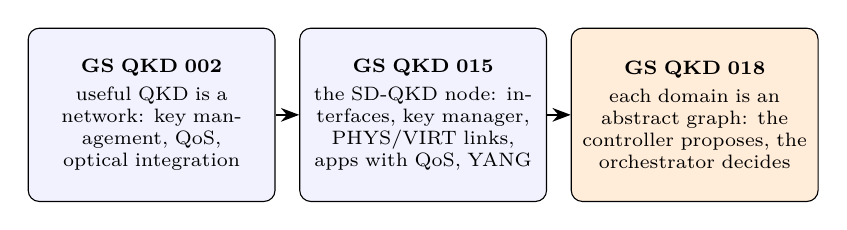
\begin{tikzpicture}[node distance=3mm,
      st/.style={draw,rounded corners,fill=blue!5,align=center,
                 font=\scriptsize,text width=2.9cm,minimum height=22mm}]
    \node[st] (a) {\textbf{GS QKD 002}\\[2pt] useful QKD is a network:
      key management, QoS, optical integration};
    \node[st,right=of a] (b) {\textbf{GS QKD 015}\\[2pt] the SD-QKD node:
      interfaces, key manager, PHYS/VIRT links, apps with QoS, YANG};
    \node[st,right=of b,fill=orange!15] (c) {\textbf{GS QKD 018}\\[2pt]
      each domain is an abstract graph: the controller proposes, the
      orchestrator decides};
    \draw[->,thick] (a) -- (b);
    \draw[->,thick] (b) -- (c);
  \end{tikzpicture}
  \end{center}
  \vspace{1ex}
  \begin{itemize}
    \item The design mirrors ACTN and reuses YANG, NETCONF and RESTCONF.
    \item Key principle: \alert{keys never leave the nodes}.
    \item KOREN, PoliMi and MadQCI: the scheme works, but orchestration is
          young. Next step: multi-operator, better metrics,
          confidentiality across domains.
  \end{itemize}
\end{frame}

\begin{frame}[allowframebreaks]{References}
  \printbibliography[heading=none]
\end{frame}

\begin{frame}
  \begin{center}
    {\Large Thank you for your attention}\\[2ex]
    Questions?
  \end{center}
\end{frame}

\end{document}
